%==================== chapter3_29.tex ====================

\clearpage
\thispagestyle{plain}

\begingroup
\fontsize{16pt}{19.2pt}\selectfont
\justifying
\XeTeXlinebreakskip=0pt plus 1pt minus 0.5pt
\setlength{\parindent}{1.5cm}
\setlength{\parskip}{0pt}

\section*{ผลการทดสอบโมเดล ResNet50}
\addcontentsline{toc}{section}{ผลการทดสอบโมเดล ResNet50}

\indent โมเดลที่ใช้ทดลองคือ ResNet50 โดยเปลี่ยนชั้นสุดท้ายให้รองรับ 3 คลาสและทำการ
Fine-tune ด้วย Optimizer แบบ AdamW พร้อม Cosine learning rate schedule และ Early
Stopping เพื่อป้องกัน Overfitting

\begin{sloppypar}
	\begin{enumerate}
		\item ค่า \textbf{Accuracy} บนชุด Validation สูงสุด = 1.0000
		\item ค่า \textbf{Macro-F1} บนชุด Validation สูงสุด = 1.0000
	\end{enumerate}
\end{sloppypar}

\indent การหยุดการฝึกเกิดขึ้นที่ Epoch 20 จากทั้งหมด 30 Epoch ตามเกณฑ์ Early Stopping กราฟการเรียนรู้ แสดงดังรูป ซึ่งเห็นได้ว่าค่า Loss ลดลงต่อเนื่องและ Accuracy
F1-score ของ Validation set เพิ่มขึ้นจนถึง 100\% นอกจากนี้ยังได้สร้าง Confusion Matrix ดังรูป ซึ่งผลลัพธ์แสดงว่าโมเดลสามารถจำแนกได้ถูกต้องครบทุกตัวอย่างในชุด Validation

\vspace{\baselineskip}

\section*{สรุปผลการทดสอบแบบจำลอง}
\addcontentsline{toc}{section}{สรุปผลการทดสอบแบบจำลอง}
\indent โมเดลสามารถจำแนกปลากัดทั้งสามกลุ่ม (ปลากัดพื้นบ้านภาคอีสานหางลาย, ปลากัดพื้นบ้านภาคใต้, ปลากัดพื้นบ้านมหาชัย) ได้อย่างถูกต้องบน
Validation set อย่างไรก็ตาม ขนาดข้อมูลยังค่อนข้างเล็กโดยเฉพาะคลาส ปลากัดพื้นบ้านมหาชัย ที่มีจำนวน
น้อย ซึ่งอาจทำให้โมเดลมี Bias และค่า Accuracy ที่ได้สูงอาจสะท้อน Overfitting ต่อโดเมนข้อมูล
ที่ใช้ ดังนั้นควรมีการทดสอบเพิ่มเติมกับชุดข้อมูลใหม่ที่ไม่ได้อยู่ในกระบวนการฝึก เพื่อประเมินความ
สามารถทั่วไป (generalization) ของโมเดล

\vspace{\baselineskip}

\begin{figure}[h]
	\centering
	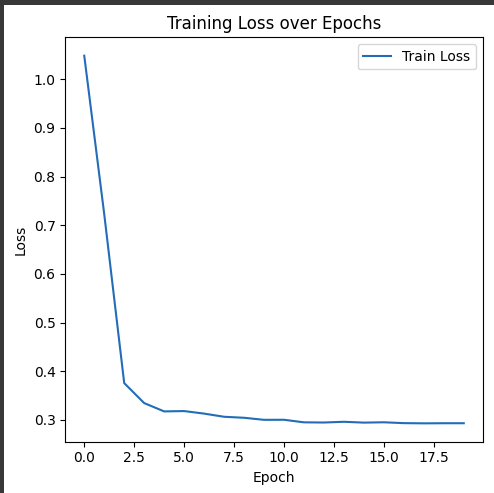
\includegraphics[width=0.47\linewidth]{GF2}
	\hfill
	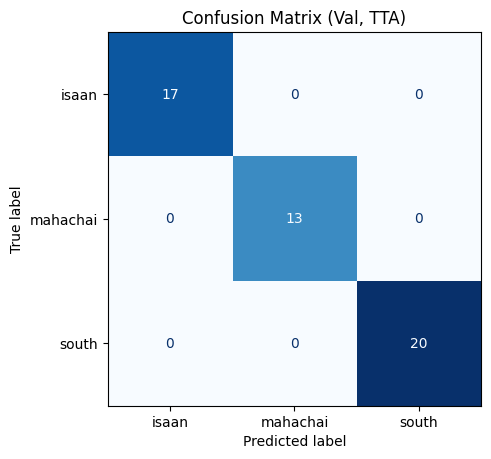
\includegraphics[width=0.47\linewidth]{GF1}
	\caption{กราฟ Loss ของ Train และ Validation และ Confusion Matrix ของผลการทดสอบ}
\end{figure}

\endgroup


